\documentclass[USenglish,oneside,twocolumn]{article}

\usepackage[utf8]{inputenc}%(only for the pdftex engine)
\usepackage[big]{dgruyter_NEW}

\usepackage{url}
\usepackage{listings}
\usepackage{caption}
\usepackage{subcaption}
\usepackage{paralist}
\usepackage{textcomp}
\usepackage{xspace}
\usepackage{ifthen}
\usepackage{amsmath}
\usepackage{color}
\usepackage{amssymb}
\usepackage{tikz}
\usetikzlibrary{arrows}
\usepackage[absolute]{textpos}
\usepackage{hyperref}
\usepackage{algorithm}
\usepackage[noend]{algpseudocode}
\usepackage{tabularx, booktabs}
\usepackage{array}
\usepackage{colortbl}
\usepackage{dcolumn}
\usepackage{adjustbox}
\usepackage{listings}
\usepackage[bottom]{footmisc}
\usepackage{cancel}
\usepackage{multirow}
\usepackage{xspace}
\usepackage{longtable}
\usepackage{balance}

\graphicspath{ {./figures/} }

\newcommand{\system}{RAN}
\newcommand{\ie}{{\em i.e.}}
\newcommand{\eg}{{\em e.g.}}
\newcommand{\ea}{{\em et al.}}

%\clubpenalty=10000  % Don't allow orphans
%\widowpenalty=10000 % Don't allow widows

\def\checkmark{\tikz\fill[scale=0.4](0,.35) -- (.25,0) -- (1,.7) -- (.25,.15) -- cycle;} 
\newtheorem{finding}{Finding}[section]
\lstdefinelanguage{JavaScript}{
  keywords={typeof, new, true, false, catch, function, return, null, catch, switch, var, if, in, while, do, else, case, break},
  keywordstyle=\color{blue}\bfseries,
  ndkeywords={class, export, boolean, throw, implements, import, this},
  ndkeywordstyle=\color{darkgray}\bfseries,
  identifierstyle=\color{black},
  sensitive=false,
  comment=[l]{//},
  morecomment=[s]{/*}{*/},
  commentstyle=\color{purple}\ttfamily,
  stringstyle=\color{red}\ttfamily,
  morestring=[b]',
  morestring=[b]"
}
 
%\DOI{foobar}
  
\begin{document}
 

  %\author[1]{Corresponding Author}

  %\author[2]{Second Author}

  %\author[3]{Third Author}

  %\author[4]{Fourth Author}

  %\affil[1]{Affil, E-mail: email@email.edu}

  %\affil[2]{Affil, E-mail: email@email.edu}

  %\affil[3]{Affil, E-mail: email@email.edu}

  %\affil[4]{Affil, E-mail: email@email.edu}

  \title{\Large \bf \system{}: Routing Around Nation-States}

  \runningtitle{\system{}: Routing Around Nation-States}

  %\subtitle{...}

\begin{abstract}
An increasing number of countries are passing laws that facilitate the
mass surveillance of their citizens. In response, governments and
citizens are increasingly paying attention to the countries that their
Internet traffic traverses. In some cases, countries are taking extreme
steps, such as building new IXPs and encouraging local interconnection
to keep local traffic local. We find that although many of these efforts
are extensive, they are often futile, due to the inherent lack of
hosting and route diversity for many popular sites. First, we characterize 
transnational routing detours by measuring the country-level paths to 
popular domains.  Then, we investigate how
the use of overlay network relays and the DNS open resolver
infrastructure can prevent traffic from traversing certain jurisdictions. 
We find that current traffic is traversing known surveillance states, but 
also show that there are tools that can be used for country avoidance. Our 
results show that 84\% of paths originating in Brazil traverse the United States, 
but when relays are used for country avoidance, only 37\% of Brazilian paths 
traverse the United States.  Unfortunately, we also find that 
some of the more prominent surveillance states are also some of the least avoidable 
countries.
\end{abstract}


%  \keywords{keywords, keywords}
%  \classification[PACS]{}
 % \communicated{...}
 % \dedication{...}

%  \journalname{Proceedings on Privacy Enhancing Technologies}
%\DOI{Editor to enter DOI}
%  \startpage{1}
%  \received{..}
%  \revised{..}
%  \accepted{..}

%  \journalyear{..}
%  \journalvolume{..}
%  \journalissue{..}
 

\maketitle
\section{Introduction}
\label{intro}

There are no restrictions on which national jurisdictions BGP paths must or must not cross.  There is also no way for an Internet user to know or decide which countries her Internet traffic is transitting.  Internet routing is usually studied at the AS (Autonomous System) level - not the nation-state level.  An AS typically controls traffic as it transits it's internal network and then defines policies for filtering, monitoring, and routing traffic to the next AS.  It is becoming increasingly common for governments to require certain actions of ASes, such as enabling wiretapping or performing censorship.  Once Internet traffic enters a country, it is subject to that country's requirements, and subsequently the corresponding ASes' actions.  More and more countries are either trying or have already passed laws that allow for mass surveillance on their citizens~\cite{france_surveillance, netherlands_surveillance, kazak_surveillance}.  Recently, the Investigatory Powers Bill (IP Bill) in the UK, if passed, will require ISPs to store citizens' browsing history for a year, and allow intelligence agencies to collect bulk data on their citizens~\cite{uk_bill}.

Currently, governments are becoming more suspicious about where their citizens' traffic is going, and are facing the challenge of controlling which countries transit the traffic.  Governments and users have been motivated more than ever since the Snowden revelations to avoid countries known for surveillance practices, specifically the United States~\cite{russia_secure_internet, routing_errors, dte}.  More recently, the Safe Harbour agreement, an agreement that allows the free flow of data between the US and the EU, was struck down because it would give the NSA access to EU citizens' personal data~\cite{safe_harbour_illegal, safe_harbour_undecided}.

In response to the Snowden revelations, Brazil has taken great measures to avoid Internet traffic from being wiretapped by the NSA~\cite{brazil_history, brazil_break_from_US, brazil_conference, brazil_conference2, brazil_human_rights}.  Some of the actions that have been taken to avoid NSA surveillance include: building a 3,500 mile long fiber-optic cable from Fortaleza to Portugal (with no use of American vendors), pressing companies such as Google, Facebook, and Twitter (among others) to store data locally, switching its dominant email system (Microsoft Outlook) to a state-developed system called Expresso~\cite{brazil_cable, brazil_us_companies}.  In other efforts, Brazil has been building Internet eXchange Points, which help grow Internet connectivity and performance~\cite{brazil_IXP1, brazil_IXP2}; it also allows them to increase their connectivity with many other countries.  Brazil now has the largest national ecosystem of public Internet eXchange points in the world~\cite{brazil_ixp_ecosystem}.  It has also been shown that over the past few years, the number of ASes in Brazil that are connected internationally have grown significantly~\cite{brazil_international_ases}.  The case of Brazil shows that countries, governments, and Internet users are motivated to avoid surveillance conducted by other countries.

Determining which countries transit Internet traffic, which countries host the only server for a given domain, and which countries are avoidable for a given domain are challenging problems.  The first challeng arises from determining the country-level path that traffic takes; paths can be collected from either the data-plane - IP-level paths - or the control-plane - AS-level paths.  Our work uses the data-plane to analyze traffic paths; in order to determine which countries are on the path, the IP-level path must be mapped to a country-level path.  This is challenging because there is no ground truth for geolocation data; there is no guarantee of accuracy or completeness.  To address this challenge, we use different geolocation tools to increase our confidence in the country-level paths we collect.  More challenges arise in determining how to avoid countries; websites are complex and can fetch data from multiple third parties, which are likely located in different geographic locations, and therefore cross different countries' borders.  The increased usage of anycast IP complicates country avoidance because it gives clients less information about the location of the server from which they are accessing content.  

In this paper, we first shed light on how much traffic is currently transiting countries known for surveillance, with a focus on the US.  Despite the measures taken by different countries to avoid the US, we still see Internet traffic that transits the US.  We conduct a measurement study that helps quantify the existing possibilities for state-sponsored surveillance.  We take Brazil as a case study, and analyze the country-level paths from machines in Brazil to the Brazil Alexa Top 100 domains.  Knowing that Brazil has taken actions to avoid traffic transitting the US, we measure how much traffic is solely transitting the US, and how much traffic is destined for the US.  These are two distinct scenarios.  If the US is solely a country on the path (and not the end point), then there is the possibility for avoiding the US.  If the domain is solely hosted in the US, and therefore destined for the US, then the US cannot be avoided for the given domain.  Using RIPE Atlas probes and the Digital Envoy geolocation service, we find that out of 36,833 traffic paths originating in Brazil to the Brazilian Alexa Top 100 domains, 2,699 are solely transitting the US and the US is the destination for 28,196 of them (this does not necessarily mean that the US is the only possible destination, but it is the destination for Brazilian Internet users)~\cite{ripe_atlas, digital_envoy}.  

Next, we present and implement a new system for surveillance circumvention for Internet users, which finally gives the users some control over where their traffic is flowing.  Because popular web companies are opening or expanding their datacenters in Europe, there are more possible paths to get data~\cite{eu_datacenters}.  It is possible that a path from a client in Brazil to a datacenter in Europe does not pass through any country known for surveillance, but may be a longer path than the best path to a datacenter in the US, as shown in Figure~\ref{fig:intro}.  Our system leverages a geographically diverse set of relay machines that act as proxies to access data from servers located in different geographic regions.  A client will first query an oracle for the best relay to use in order to avoid a given country.  Then the oracle will respond with the IP address of the best relay, which the client will then send it's request to.  The relay will fetch the data from the domain's closest server and return the data to the client. \annie{Add a couple highlights of the results/evaluation section when we get there.}

\begin{figure}
\centering
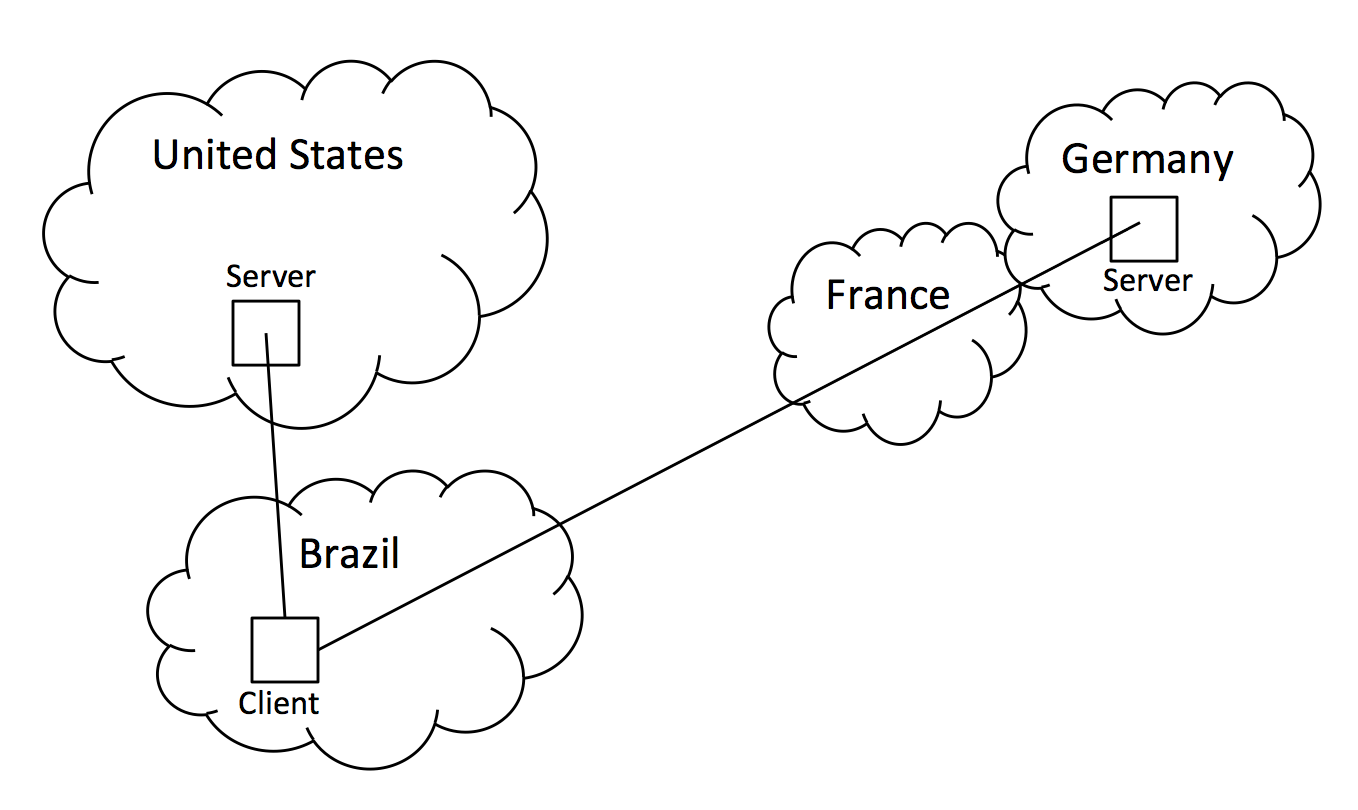
\includegraphics[width=.5\textwidth]{intro_fig}
\caption{A shorter path to a server in a country known for surveillance (U.S.), and a longer path to a georeplicated server in Germany.  The longer path may be more preferred by the client because it doesn't traverse a country with known surveillance practices.}
\label{fig:intro}
\end{figure}

This paper is organized as follows.  In the next section, we describe our research goals, and the challenges in achieving them.  In Section~\ref{datasets} we discuss how and where we collected our data.  We point out the advantages and disadvantages of existing datasets, and justify our decision.  In Section \ref{measure}, we design and execute a measurement study on the country-level paths of Brazil's Internet.  We describe our methodology, as well as results that show which countries Brazil's Internet traffic is traversing.  Next, Section \ref{architecture} introduces SYSTEM, which allows Internet users, ISPs, and Internet services to avoid specified countries, and therefore circumvent surveillance.  Then we explain our implementation of SYSTEM in Section \ref{implementation}.  In Section \ref{evaluation}, we evaluate our system and proposed methods for how well they avoid any given country.  We discuss how our system differs from others and uniquely suits the purpose of country avoidance in Section \ref{discussion}, we review related work in Section \ref{related}, and conclude in Section \ref{conclusion}.

\section{Related Work}
\label{related}

\paragraph{Nation-state routing analysis.}  Shah and
Papadopoulos recently measured international routing detours---paths that originate
in
one country, cross international borders, and then return to the
original country)---using public Border Gateway Protocol~(BGP) routing tables~\cite
{shah2015characterizing}. 
The study discovered 2 million detours each month out
of 7 billion total paths); the study also characterized the detours based
on detour dynamics and persistence.  Our work differs because it {\em actively}
measures traceroutes, yielding a more precise measurement of the path traffic is
likely to take, as opposed to analyzing BGP
routes.  Obar and Clement analyzed traceroutes
that started and ended in Canada, but tromboned through the United
States, and argued that
this is a violation of Canadian network
sovereignty~\cite{obar2012internet}. 
Karlin \ea developed a framework for country-level
routing analysis to study how much influence each country has over
interdomain routing~\cite{karlin2009nation}.  This work measures the
centrality of a country using BGP routes and AS-path inference; in contrast, our work uses active 
measurements and measures avoidability of a given country. 

\paragraph{Mapping national Internet topologies.}  Roberts \ea developed a method
for mapping national networks of ASes, identifying ASes that act as points of
control~\cite{roberts2011mapping}.   %JEN: not clear we care about the
"complexity" (whatever that means) %, and measuring the complexity of the
national network Several studies have also characterized network paths {\em
within} a country, including
Germany~\cite{wahlisch2010framework,wahlisch2012exposing} and
China~\cite{zhou2007chinese}, or a country's interconnectivity within a region
or with the rest of the
world~\cite{bischof2015and,gupta2014peering,fanou2015diversity}; these studies
focus on paths within a country of interest, as opposed to focusing on
transnational Internet paths.

\paragraph{Routing overlays and Internet architectures.} Alibi Routing uses
round-trip times to prove that that a client's packets did  not traverse a
forbidden country or region~\cite{levin2015alibi}; our work differs by
measuring  which countries a client's packets would (and does) traverse.  Our
work then  uses active measurements to determine the best path for a client
wishing  to connect to a server.  RON, Resilient Overlay Network, is an
overlay network that  routes around failures, whereas our overlay network
routes around countries~\cite{andersen2001resilient}.  ARROW introduces a
model that allows users to route around ISPs~\cite{peter2015one}, but requires
ISP participation, making it considerably more difficult to deploy than
\system{}. ARROW also aims to improve fault-tolerance, robustness, and
security, rather than explicitly attempting to avoid certain countries; ARROW
provides mechanisms to avoid individual ISPs, but such a mechanism is at a
different level of granularity, because an ISP may span multiple countries.
Zhang \ea presented SCION, a ``clean-slate'' Internet architecture that
provides route control, failure isolation, and explicit trust information for
communication~\cite{zhang2011scion}; SCION, however, requires fundamental
changes to the Internet architecture, whereas \system{} is deployable today.


\paragraph{Circumvention systems.}  Certain tools, such as anonymous
communications systems or virtual private networks, may use a combination of
encryption and overlay routing to allow clients to avoid surveillance. Tor is
an anonymity system that uses three relays and layered encryption to allow
users to communicate anonymously~\cite{dingledine2004tor}.  In contrast,
\system{} does not aim to achieve anonymity; instead, its aim is to ensure
that traffic does not traverse a specific  country, a goal that Tor cannot
achieve.  Even tools like Tor do not inherently thwart surveillance: Tor is
vulnerable to traffic correlation attacks and some attacks are possible even
on encrypted user traffic. VPNGate is a public VPN relay system aimed at
circumventing national firewalls~\cite{nobori2014vpn}. Unfortunately, VPNGate
does not allow a client to choose any available VPN, which makes it more
difficult for a user to ensure that traffic avoids a particular part of the
Internet.  Neither of these systems explicitly avoid countries; thus, they may
not  be able to avoid surveillance or the laws or jurisdiction of a particular
country. Additionally, existing circumvention systems generally rely on
encryption, which does not prevent surveillance; prior research has shown that
websites can be fingerprinted based on size, content, and location of third
party resources, which  reveals information about the content a user is
accessing \cite{what_isps_can_see}.  Finally, ISPs often execute man-in- the-
middle attacks on TLS connections to perform network management
functions~\cite{mitm_isp}.


\section{Characterizing Transnational Detours}
\label{datasets}
In this section, we describe our measurement methods, the challenges in
conducting them, and our findings concerning the transnational detours
of default Internet paths.

\begin{figure*}[t]
\centering
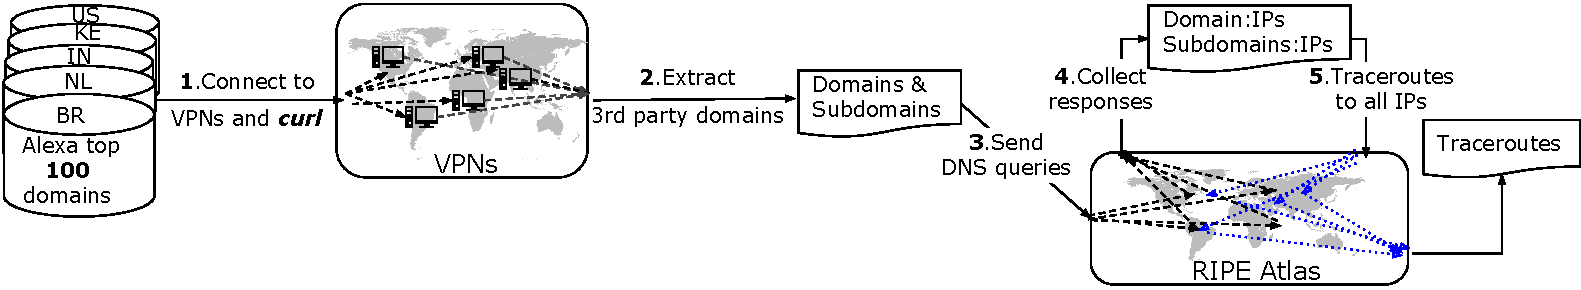
\includegraphics[width=.9\textwidth]{Current-Traffic_fig}
\caption{Measurement pipeline to study Internet paths from countries to
  popular domains.}
\label{fig:pipeline1}
\end{figure*}


\subsection{Measurement Approach and Challenges}
\label{pipeline}

\paragraph{Overview of approach.}
Figure~\ref{fig:pipeline1} shows the process that we use to discover end-to-end
Internet paths from our respective vantage points to various domains. We first use
VPNs
to establish various vantage points in the countries of interest; then, we use 
{\tt curl} to download corresponding webpages for each of those popular domains,
including all subdomains that are embedded in the site's top-level webpage. We extract
all of these domain names and resolve them to their corresponding IP addresses;
we then perform traceroutes to each of those IP addresses.
Figure~\ref{fig:analysis_pipeline} describes how we translate an IP-level traceroute
to a country-level path. We geolocate each IP address, removing unknown hops; we
then de-duplicate the country-level path. Although it is seemingly straightforward,
this approach entails a number of limitations and caveats, which we describe in
the
rest of this section.
%JEN: repetitive
%Using traceroutes to measure
%transnational detours is new; prior work used BGP routing tables to
%\textit{infer} country-level paths~\cite{karlin2009nation}.  

\subsubsection{Resource Limitations}
\label{resource_limits}

We currently focus our measurements on twenty countries due to resource limitations.
The iPlane~\cite{madhyastha2006iplane} and Center for Applied Internet Data
Analysis (CAIDA)~\cite{caida} projects maintain large repositories of
traceroute data, neither of which are suitable for our study.   iPlane has
historical data as far back as 2006. Unfortunately, because iPlane uses
PlanetLab~\cite{PlanetLab} nodes, which are primarily hosted on the Global
Research and Education Network (GREN), iPlane measurements are not be
representative of typical Internet users' traffic
paths~\cite{banerjee2004interdomain}.  CAIDA runs traceroutes from different
vantage points around the world to randomized destination IP addresses that
cover all /24s; in contrast, we focus on paths to popular websites from a
particular country.

Instead, we run active measurements that
intend to better represent paths of a typical Internet user. To do so, we run
DNS and traceroute measurements from RIPE Atlas probes, which are hosted
all around the world in many different types of networks, including home
networks~\cite{ripe_atlas}.  RIPE Atlas probes can use the local DNS
resolver, which would give us the best estimate of the traceroute
destination.  

Conducting measurements from a RIPE Atlas probe costs a certain
amount of ``credits'', which restricts the number of measurements that we
could run.  RIPE Atlas also imposes rate limits on the number of
concurrent measurements and the number of credits that an individual
user can spend per day.  We address these challenges in two ways: (1)~we
reduce the number of necessary measurements we must run on RIPE Atlas
probes by conducting traceroute measurements to a single IP address in
each /24 (as opposed to all IP addresses returned by DNS) because all IP
addresses in a /24 belong to the same AS, and should therefore be
located in the same geographic area; (2)~we use a different method---VPN
connections---to obtain a vantage point within a foreign country, which
is still representative of an Internet user in that country.

\subsubsection{Path Asymmetry}
\label{path_sym}

The reverse path is just as important as (and often different from) the
forward path.   Previous work has shown that paths between Internet endpoints
are often asymmetric~\cite{he2005routing}.  Most work on path asymmetry has
been done at the AS level, but not at the country level; our measurements can
consider only the forward path (from client to domain or relay), not the
reverse path from the domain or relay to the client.

To better understand the limitation of our current measurements, we also (separately)
measured path asymmetry at the country granularity. If country-level paths
were symmetric, then the results of our measurements would be representative
of the forward {\it and} reverse paths. If the country-level paths are
asymmetric, then our measurement results only provide a lower bound on the
number of countries that traffic between two endpoints may traverse.  Using
100 RIPE Atlas probes located around the world and eight Amazon EC2 instances,
we ran traceroute measurements from every probe to every EC2 instance and from
every EC2 instance to every probe.  After mapping the IPs to countries, we
analyzed the paths for symmetry.  First, we compared the set of countries on
the forward path to the set of countries on the reverse path; this yielded
about 30\% symmetry.  We compared the number of countries on the forward and
reverse paths to determine how many reverse paths were a subset of the
respective forward path; this situation occurred for 55\% of the paths. This
level of asymmetry suggests that our results represent a lower bound on the
number of countries that transit traffic; our results are a lower bound on how
many unfavorable countries transit a client's path. It also suggests that
while providing lower bounds on transnational detours is feasible, designing
systems to {\em completely} prevent these detours on both forward and reverse
paths is extremely challenging. If tools that shed light on the reverse path
between endpoints (\eg, Reverse Traceroute) see more widespread deployment,
the characterizations and avoidance techniques that we develop in this paper could
be extended to include reverse paths.

\subsubsection{Traceroute Origin and Destination Selection}

Each country hosts a different number of RIPE Atlas probes, ranging
from roughly 75 probes to several hundred probes.  Because of the resource
restrictions, we could not use all of the probes in each country.  We
selected the set of probes that had unique ASes in the country to get
the widest representation of origination (starting) points.

We used the Alexa Top 100 domains in each of the respective countries as our
destinations, as well as the third-party domains that are requested as part of
an original web request.  For a smaller set of vantage points, we compared the
country-level paths to the top 100 domains and to those from the vantage
points to the top 1000 domains. The proportion of paths that transited (and
ended in) each country are similar in both cases; the paths to the top 1000
domains exhibit a longer tail of countries that transit or host content,
likely because these domains are less popular and therefore hosted in more
obscure locations. Otherwise, the results are similar.

To obtain the third-party domains that are hosted on each popular website, we
use {\tt curl} to retrieve the homepage for each respective domain from within
the country that is hosting the vantage point in question.  RIPE Atlas probes
do not support these types of Web requests; instead, we establish a VPN
connection within each of these countries to {\tt curl} each domain and
extract the third-party domains; we {\tt curl} from the client's location in
case web sites are customizing content based on the region of the client.

\begin{figure}[t]
\centering
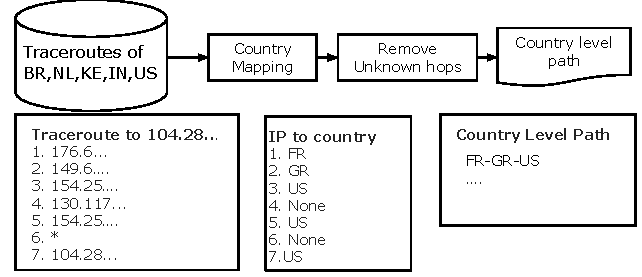
\includegraphics[width=.5\textwidth]{Analysis-Pipeline1}
\caption{Mapping country-level paths from traceroutes.}
\label{fig:analysis_pipeline}
\end{figure}


\subsubsection{Country Mapping}
\label{c_map}

Accurate IP geolocation is challenging. We use MaxMind's
geolocation service to map IP addresses to their respective
countries~\cite{maxmind}. Unfortunately, this database is known to contain inaccuracies,
particularly for IP addresses that correspond to Internet infrastructure, as opposed
to end hosts.
Fortunately, previous
work has found that
geolocation at a country-level granularity is more accurate than at
finer granularity~\cite{huffaker2011geocompare}.  In light of these
concerns, we post-processed our IP to country mapping
by removing all IP addresses that resulted in a `None' response when
querying MaxMind, which causes our results to provide a conservative
estimate of the number of countries that paths traverse. It is important
to note that removing `None' responses will \textit{always} produce a
conservative estimate.
%JEN: removed to deemphasize surveillance as the primary interest
%, and therefore we are \textit{always}
%underestimating the amount of potential surveillance.  
Figure~\ref{fig:analysis_pipeline} shows an example of this
post-processing. 

\subsection{Results}


%%%% ADD THIS TO datasets.tex
\newcolumntype{d}[1]{D{.}{.}{#1}}
\newcommand{\headrow}[1]{\multicolumn{1}{c}{\adjustbox{angle=45,lap=\width-0.5em}{#1}}}
\newcolumntype{P}[1]{>{\raggedright\arraybackslash}p{#1}}
\newcommand{\ra}[1]{\renewcommand{\arraystretch}{#1}}
\begin{table}[t]
\centering
\ra{1}
\resizebox{\columnwidth}{!}{%
\begin{tabular}{@{}ld{3.2}d{3.2}d{3.2}d{3.2}d{3.2}@{}}
%\multicolumn{1}{l}{}    & \headrow{Host} & \headrow{Transit} & \headrow{Host} & \headrow{Transit} &\headrow{Host} &\headrow{Transit} &\headrow{Host}   &\headrow{Transit} &\headrow{Host}  &\headrow{Transit} \\
\textit{Terminating in Country} 
   & \headrow{Brazil}  & \headrow{Netherlands}   & \headrow{India} & \headrow{Kenya} & \headrow{United States}\\
\toprule
Brazil             &.169    &\multicolumn{1}{r}{-}     &\multicolumn{1}{r}{-}    &\multicolumn{1}{r}{-}  &\multicolumn{1}{r}{-} \\ \midrule
Canada             &.001    &.007     &.015      &.006       &\multicolumn{1}{r}{-}  \\
United States      &\cellcolor[HTML]{F7BE81}.774    &\cellcolor[HTML]{F7BE81}.454      &\cellcolor[HTML]{F7BE81}.629      &\cellcolor[HTML]{F7BE81}.443        &\cellcolor[HTML]{F7BE81}.969    \\ \midrule
France             &.001    &.022      &.009      &.023       &.001 \\
Germany            &.002    &.013      &.014      &.028       &.001  \\
Great Britain      &\multicolumn{1}{r}{-}  &.019     &.021     &.032       &.002 \\
Ireland            &.016    &.064      &.027       &.108       &.001   \\
Netherlands        &.013    &\cellcolor[HTML]{F7BE81}.392      &\cellcolor[HTML]{F7BE81}.101      &\cellcolor[HTML]{F7BE81}.200      &.024  \\
Spain              &.001    &\multicolumn{1}{r}{-}     &\multicolumn{1}{r}{-}    &\multicolumn{1}{r}{-}     &\multicolumn{1}{r}{-}    \\ \midrule
Kenya              &\multicolumn{1}{r}{-}        &\multicolumn{1}{r}{-}    &\multicolumn{1}{r}{-}    &.022        &\multicolumn{1}{r}{-}  \\
Mauritius          &\multicolumn{1}{r}{-}      &\multicolumn{1}{r}{-}    &\multicolumn{1}{r}{-}   &.004       &\multicolumn{1}{r}{-}  \\
South Africa       &\multicolumn{1}{r}{-}       &\multicolumn{1}{r}{-}     &\multicolumn{1}{r}{-}  &.021       &\multicolumn{1}{r}{-}  \\ \midrule
United Arab Emirates &\multicolumn{1}{r}{-}     &\multicolumn{1}{r}{-}     &\multicolumn{1}{r}{-}   &.011        &\multicolumn{1}{r}{-}  \\
India              &\multicolumn{1}{r}{-}      &\multicolumn{1}{r}{-}     &.053    &.002        &\multicolumn{1}{r}{-}  \\
Singapore          &\multicolumn{1}{r}{-}       &.002     &\cellcolor[HTML]{F7BE81}.103      &.027       &\multicolumn{1}{r}{-} \\\hline
\end{tabular}
}
\caption{Fraction of paths that terminate in each country by default.}
\label{tab:host}
\end{table}

\begin{table}[t]
\centering
\ra{1}
\resizebox{\columnwidth}{!}{%
\begin{tabular}{@{}ld{3.2}d{3.2}d{3.2}d{3.2}d{3.2}@{}}
%\multicolumn{1}{l}{}    & \headrow{Host} & \headrow{Transit} & \headrow{Host} & \headrow{Transit} &\headrow{Host} &\headrow{Transit} &\headrow{Host}   &\headrow{Transit} &\headrow{Host}  &\headrow{Transit} \\

\textit{Transiting Country}    & \headrow{Brazil}  & \headrow{Netherlands}   & \headrow{India} & \headrow{Kenya} & \headrow{United States}\\ \toprule
Brazil              &1.00       &\multicolumn{1}{r}{-}   &\multicolumn{1}{r}{-}     &\multicolumn{1}{r}{-}     &\multicolumn{1}{r}{-} \\ \midrule
Canada                &.013       &.007     &.016       &.008      &.081 \\
United States        &\cellcolor[HTML]{F7BE81}.844        &\cellcolor[HTML]{F7BE81}.583     &\cellcolor[HTML]{F7BE81}.715      &\cellcolor[HTML]{F7BE81}.616       &\cellcolor[HTML]{F7BE81}1.00 \\ \midrule
France                 &.059     &.102      &.104       &.221      &.104 \\
Germany                 &.005       &.050    &.032      &.048      &.008 \\
Great Britain                &.024       &\cellcolor[HTML]{F7BE81}.140     &\cellcolor[HTML]{F7BE81}.204      &\cellcolor[HTML]{F7BE81}.500      &.006 \\
Ireland                &.028       &.106      &.031     &.133      &.006 \\
Netherlands                 &.019        &1.00      &.121      &\cellcolor[HTML]{F7BE81}.253      &.031 \\
Spain                  &.176       &.004     &\multicolumn{1}{r}{-}     &\multicolumn{1}{r}{-}      &\multicolumn{1}{r}{-} \\ \midrule
Kenya                 &\multicolumn{1}{r}{-}       &\multicolumn{1}{r}{-}    &\multicolumn{1}{r}{-}      &1.00      &\multicolumn{1}{r}{-} \\
Mauritius                  &\multicolumn{1}{r}{-}       &\multicolumn{1}{r}{-}     &\multicolumn{1}{r}{-}      &\cellcolor[HTML]{F7BE81}.322       &\multicolumn{1}{r}{-} \\
South Africa                 &\multicolumn{1}{r}{-}        &\multicolumn{1}{r}{-}    &\multicolumn{1}{r}{-}     &\cellcolor[HTML]{F7BE81}.334       &\multicolumn{1}{r}{-} \\ \midrule
United Arab Emirates                  &\multicolumn{1}{r}{-}        &\multicolumn{1}{r}{-}    &\multicolumn{1}{r}{-}     &.152       &\multicolumn{1}{r}{-} \\
India               &\multicolumn{1}{r}{-}    &\multicolumn{1}{r}{-}    &1.00     &.058     &\multicolumn{1}{r}{-} \\
Singapore                 &\multicolumn{1}{r}{-}        &.002     &\cellcolor[HTML]{F7BE81}.270       &.040       &.003 \\ \midrule
\end{tabular}
}
\caption{Fraction of paths that each country transits by default.}
\label{tab:transit}
\end{table}


Table~\ref{tab:host} shows five of the countries that we studied along the top
of the table and the countries that host their content along in each row.  A
``-'' represents the case where no paths ended in that country. For example,
the United States is the endpoint of 77.4\% of the paths that originate in
Brazil, and no Brazilian paths terminated in South Africa.
Table~\ref{tab:transit} shows the fraction of paths that transit (or end in)
certain countries, with a row for each country that is transited.

\begin{finding}[Hosting Diversity] About half of the top domains in each of
the five countries studied are hosted in a single country.  The other half are
located in two or more different countries. \end{finding} 

\noindent First, we analyze hosting diversity, which reveals how many unique
countries host a domain.  The more countries host a domain, the greater the
likelihood that a client can find a path to that site that avoids a certain
country. As a separate measurement experiment, we queried DNS from 26 vantage points around the world, in
geographically diverse locations. We then mapped the IP addresses in the DNS
responses to countries to determine how many unique countries host a domain.
Figure~\ref{fig:host_diversity} shows the fraction of domains that are hosted
in different numbers of countries; we can see two common hosting cases:
(1)~CDNs and (2)~a single hosting country.  This shows that many domains are
hosted in a single unique country, which leads us to our next analysis---where
are these domains hosted, and which countries are traversed on the way to
reach these locations.

%\begin{figure}[t]
%\centering
%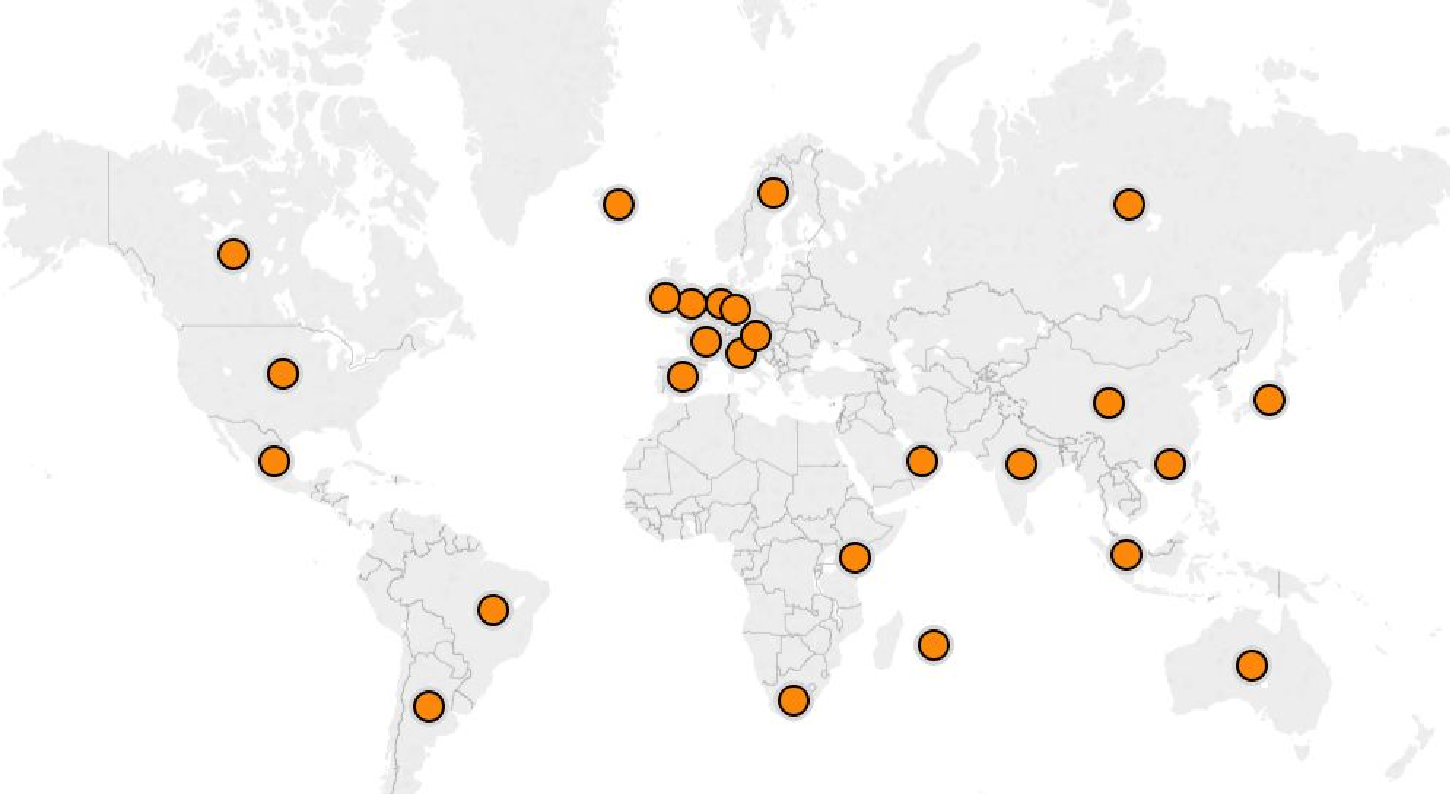
\includegraphics[width=0.8\columnwidth]{World-DNS}
%\caption{Vantage points in measuring hosting diversity.}
%\label{fig:world}
%\end{figure}

\begin{figure}[t]
\centering
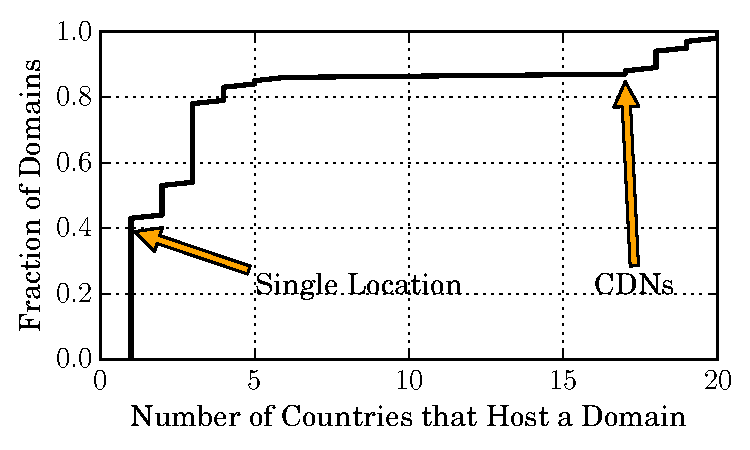
\includegraphics[width=.8\columnwidth]{domain_hist_US1}
\caption{The number of Alexa Top 100 US Domains hosted in different countries.}
\label{fig:host_diversity}
\end{figure}


\begin{figure*}[t!]
\begin{minipage}{\linewidth}
\begin{subfigure}[b]{.32\linewidth}
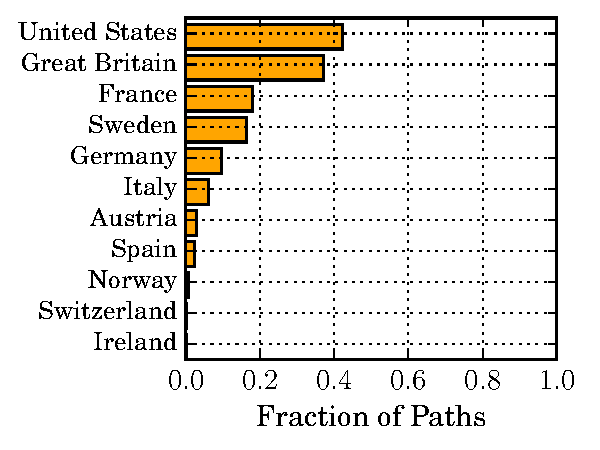
\includegraphics[width=\linewidth]{nl_trombone_new11}
\caption{The Netherlands.\label{fig:trombone_netherlands}}
\end{subfigure}
\begin{subfigure}[b]{.32\linewidth}
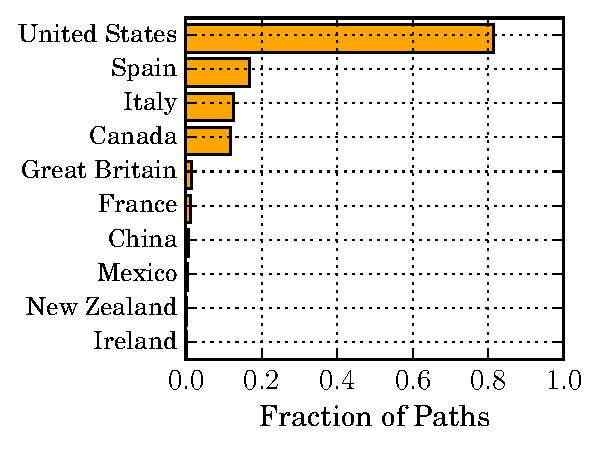
\includegraphics[width=\linewidth]{br_trombone_new11}
\caption{Brazil.\label{fig:trombone_brazil}}
\end{subfigure}
\begin{subfigure}[b]{.32\linewidth}
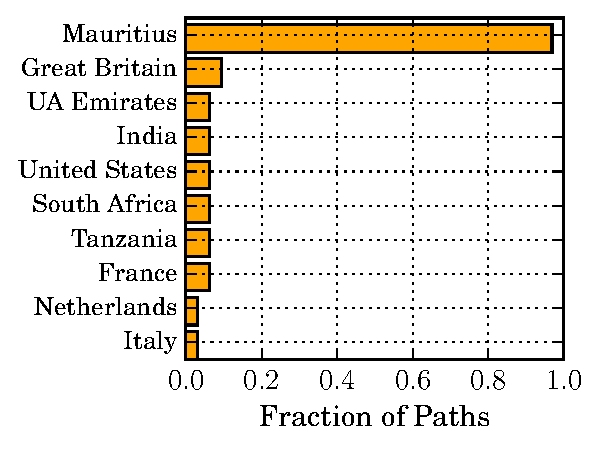
\includegraphics[width=\linewidth]{ke_trombone_new11}
\caption{Kenya.\label{fig:trombone_kenya}}
\end{subfigure}
\end{minipage}
\caption{The countries that tromboning paths from the Netherlands, Brazil, and Kenya transit.}
\label{fig:trombone}
\end{figure*}



\begin{finding}[Domain Hosting]
The most common destination, regardless of originating country, is the United States:
77\%, 45\%, 63\%, 44\%, and 97\% of paths originating in Brazil, Netherlands, India,
Kenya,
and the United States, respectively, are currently reaching content located in the
United States.
\end{finding}
\noindent
Table~\ref{tab:host} shows the fraction of paths that are hosted in various
countries.  Despite the extent of country-level hosting diversity, the
majority of paths from all of the countries we studied terminate in a single
country: the United States, a known surveillance state.   Our results also
show the Netherlands is a common hosting location for paths originating in the
Netherlands, India, and Kenya.

%For Indian traffic, in addition to the 63\% hosted in the United States and the 10\% hosted in the Netherlands, another 10\% is hosted in Singapore.  Hosting in these countries can best be explained by the number of underwater cables with landing points in both India and Singapore~\cite{cablemap}.  More specifically, there is a cable that directly connects Chennai, India and Changi North, Singapore, and is owned by Tata Communications, which is one of the top global Internet providers (in terms of transited IP space)~\cite{bakers}.  

%For Kenyan traffic, the United States hosts 44\% of the content, but Ireland hosts 10\%; Ireland is a popular hosting location for U.S. companies due to its relaxed enforcement of privacy in the private sector \annie{I got this information from Joel Reidenberg - how do I cite that?  I'll also look to see if I can find any publications that discuss this}.  

\begin{finding}[Domestic Traffic]
All of the countries studied (except for the United States) host content for a small percentage of the paths that originate in their own country; they also host a small percentage of their respective country-code top-level domains.
\end{finding}
\noindent
Only 17\% of paths that originate in Brazil also end there.  Only 5\%
and 2\% of Indian and Kenyan paths, respectively, end in the originating
country.  
For Kenya, 24 out of the Top 100 Domains are .ke domains, but only 5
of the 24 are hosted within Kenya.  29 out of 40 .nl domains are hosted in the Netherlands;
four of 13 .in domains are hosted in India; 18 of 39 .br domains are hosted in Brazil.
Interestingly, all .gov domains were hosted in their respective country. 

\begin{finding}[Transit Traffic]
The United States and Great Britain are on the largest portion of paths in comparison to any other (foreign) country.
\end{finding}
\noindent
84\% of Brazilian paths traverse the United States, despite Brazil's
strong efforts to avoid United States surveillance.  Although India and
Kenya are geographically distant, 72\% and 62\% of their paths also transit
the United States.

Great Britain and the Netherlands are on 
many of the paths from Kenya and India:
50\% and 20\% of
paths that originate in Kenya and India, respectively, transit Great
Britain.   Many paths likely traverse Great Britain and the Netherlands due to
the presence of large Internet Exchange Points (\ie, LINX, AMS-IX).
Mauritius, South Africa, and the United Arab Emirates transit 32\%,
33\%, and 15\% of paths from Kenya.  There are direct underwater cables
from Kenya to Mauritius, and from Mauritius to South
Africa~\cite{cablemap}.  Additionally, a cable from Mombasa,
Kenya to Fujairah, United Arab Emirates likely explains why many
paths include these countries. 



\begin{finding}[Tromboning Traffic]
Brazilian and Netherlands paths often trombone to the United States, despite the prevalence of IXPs in both countries.
\end{finding}
\noindent
Figure~\ref{fig:trombone}
shows the fraction of paths that trombone to
different countries for the Netherlands, Brazil, and Kenya. 24\% of
all paths originating in the Netherlands (62\% of domestic paths)
trombone to a foreign country before returning to the
Netherlands. Despite Brazil's strong efforts in building IXPs to keep
local traffic local, 
their paths still trombone to the U.S.  This is due to IXPs being seen
as a threat by competing commercial providers; providers are sometimes
concerned that ``interconnection'' will result in making business
cheaper for competitors and stealing of customers~\cite{ixp_policy}.

Brazilian providers likely see one another as competitors and therefore as a
threat at IXPs, which causes them to peer with international providers instead
of other local providers.  Additionally, we see Brazilian paths trombone to
Spain and Italy.  We see Italy often in tromboning paths because Telecom
Italia Sparkle is one of the top global Internet providers~\cite{bakers}. We
note that MaxMind's geolocation sometimes mislabels IP addresses to be in
Spain when they are actually located in Portugal.  Despite our inability to
disambiguate Spain and Portugal, some of the issues associated with tromboning,
such as performance, are still pertinent. We are not aware of specific laws in
either of these countries that would make this distinction important from a
policy or legal aspect, either.

Tromboning paths that originate in Kenya most commonly traverse Mauritius,
which is expected considering the submarine cables between Kenya and
Mauritius.  The topology of submarine cables may also explain why we observe
South Africa, Tanzania, and the United Arab Emirates on many tromboning paths
from Kenya.

  %Traffic that should be kept local is susceptible to surveillance because it transits two well-known surveillance states.  

\begin{finding}[United States as an Outlier]
The United States hosts 97\% of the content that is accessed from within the United States, and only five foreign countries---France, Germany, Ireland, Great Britain, and the Netherlands---host content for the other 3\% of paths.
\end{finding}
\noindent

We find that Brazilian, Dutch, Indian, and Kenyan paths
often transit the U.S. (as well as other countries that have permissive
surveillance laws). The results from
studying paths that originate in the United States are drastically different from
those
of the other four countries.  The majority of locally popular content in these countries
is hosted outside of the respective country; in contrast, the United States hosts
97\% of the
content that is accessed from within the country.  Only 13 unique countries
are ever on a path from the United States to a domain in the top 100 (or third party
domain), whereas 30, 30, 25, and 38 unique countries are seen on the paths
originating in Brazil, Netherlands, India, and Kenya, respectively.

%There are only 6 foreign countries---France, Germany, Ireland, Great Britain, and the Netherlands----that host content for traffic originating in the United States, and the fraction of content hosted in these countries is less than 4\% combined.

\subsection{Limitations}

This section discusses the various limitations of our measurement methods
and how they may affect our results.

\paragraph{Traceroute accuracy and completeness.}
Our study is limited by the accuracy and completeness of traceroute.
Anomalies can occur in traceroute-based
measurements~\cite{augustin2006avoiding}, but most traceroute anomalies
do not cause an overestimation in surveillance states.  The
incompleteness of traceroutes, where a router does not respond, causes
our results to underestimate the number of surveillance states, and
therefore also provides a lower bound on surveillance. 

\paragraph{IP geolocation vs.\ country mapping.}
There are fundamental challenges in deducing a geographic location
from an IP address, 
%JEN: remove the details about methods?
despite using different methods such as DNS names of the target,
network delay measurements, and host-to-location mapping in
conjunction with BGP prefix
information~\cite{padmanabhan2001investigation}.  While there are
inaccuracies and incompleteness in MaxMind's
data~\cite{huffaker2011geocompare}, the primary motivations for this work are to show that paths 
are currently going through surveillance states, and that performance is affected by the 
paths taken.  We use Maxmind to map IP to
country,
% (as described in Section~\ref{c_map}),
which provides a lower
bound on the amount of surveillance and tromboning.

\paragraph{IPv4 vs.\ IPv6 connectivity.}
We collect and analyze only IPv4 paths.  IPv6 paths likely
differ from IPv4 paths as not all routers that support IPv4 also support
IPv6.  A comparable study of IP-level paths is an avenue for future work.


\section{Feasibility of Routing Around Nation-States}
\label{avoid_results}

We now explore the extent to which overlay networks can improve path diversity and help clients 
route around specific countries.  We develop an avoidance metric and algorithm, and
evaluate the effectiveness of overlay nodes to avoid specific countries.

\subsection{Measurement Approach}
\label{avoid_pipelines}

An overlay network of relay nodes can
help clients route around countries or access content 
that is hosted in a different country; this section performs measurements to evaluate
the feasibility of such an approach. Figure~\ref{fig:avoidance_relays}
shows the steps in our measurement experiment.
After selecting potential relay nodes, we perform traceroute measurements from
the country of origin to each relay (1',2'), and from each relay to the set of top 100 domains
in the original country (1,2,3). We
then analyze these traceroutes using the approach shown in Figure~\ref{fig:analysis_pipeline}
to determine the resulting country-level paths. 

\begin{figure}[t]
\centering
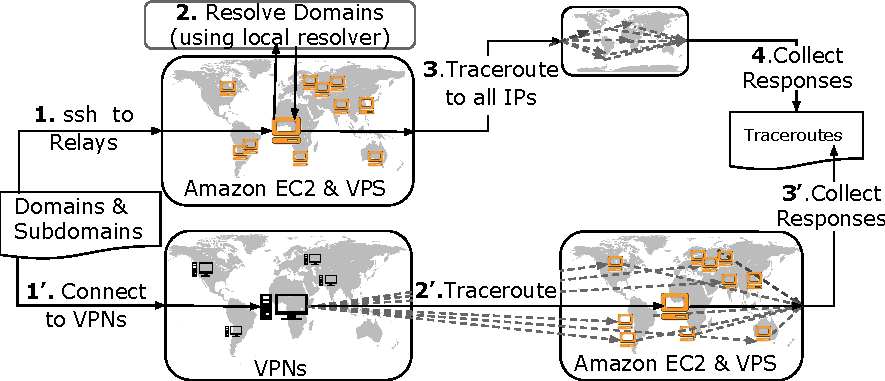
\includegraphics[width=.45\textwidth]{Country-Avoidance-Relays}
\caption{Measurement approach for country avoidance.}
\label{fig:avoidance_relays}
\end{figure}

We use eight EC2 instances, one in each region
(United States, Ireland, Germany, Singapore, South Korea, Japan, Australia,
Brazil), as well as four Virtual Private Server (VPS) machines (France,
Spain, Brazil, Singapore), which are virtual machines.
% that are functionally equivalent to dedicated physical servers.  
Combining these two sets of machines allows us to evaluate country avoidance with a diverse set of relays. 

\subsection{Avoidability Metrics}
\label{metrics}

We introduce a new metric, avoidability, to measure how often a client in
one country can avoid another specific country.
Using the proposed metric
and algorithm, we can compare how well the different methods achieve
country avoidance for any (X, Y) pair.

{\bf Avoidability metric.}  We introduce an avoidability metric to
quantify how often
traffic can avoid Country Y when it originates in Country X.
Avoidability reflects the fraction of paths that originate in Country
X and do not transit Country Y.  We calculate this value by dividing the
number of paths from Country X to domains that do not traverse Country Y
by the total number of paths from Country X. The resulting value is
in the range [0,1], where 0 means the country is unavoidable for all of
the domains in our study, and 1 means the client can avoid Country Y for
all domains in our study.  For example, there are three paths
originating in Brazil: (1)~$BR \rightarrow US$, (2)~$BR \rightarrow CO
\rightarrow None$, (3)~$BR \rightarrow *** \rightarrow BR$.  After
processing the paths as described in Section~\ref{c_map}, the resulting
paths are: (1)~$BR \rightarrow US$, (2)~$BR \rightarrow CO$, (3)~$BR
\rightarrow BR$.  The avoidance value for avoiding the United States
would be 2/3 because two out of the three paths do not traverse the
United States.  This metric represents a lower bound,
because it is possible that the third path timed out ($***$) because it
traversed the United States, which would make the third path: $BR
\rightarrow US \rightarrow BR$, and would cause the avoidance metric to
drop to 1/3.

{\bf Avoidability algorithm with relays.}  Measuring the avoidability of Country Y
from a client in Country X using relays entails two components: (1)~Is Country Y
on the path from the client in Country X to the relay?  (2)~Is Country Y on
the path from the relay to the domain?  For every domain, our algorithm checks
if there exists at least one path from the client in Country X through any
relay and on to the domain, and does not transit Country Y.   The algorithm
 produces a value in the range [0,1] that can be
compared to the output of the avoidability metric.

%{\bf Upper bound on avoidability.}  Although the avoidability metric
%provides a way to quantify how avoidable Country Y is for a client in Country
%X, some domains may be hosted only in Country Y, so the avoidance value  would
%never reach 1.0.  For this reason, we measured the {\em upper bound} on
%avoidance for a given pair of (Country X, Country Y) that represents the best
%case value for avoidance.  This algorithm analyzes the destinations of all
%domains from all relays and if there exists at least one destination for a
%domain that is not in Country Y, then this increases the upper bound value. An
%upper bound of 1.0 means that every domain that we measured is hosted (or has
%a replica) outside of Country Y.  This value puts the avoidance values in
%perspective for each (Country X, Country Y) pair.

\subsection{Results}

We examine the
effectiveness of relays for country avoidance, as well as for keeping local
traffic local.  Table \ref{tab:avoid} shows avoidance values; the top
row shows the countries we studied and the left column shows the country
that the client aims to avoid.
%
Table \ref{tab:avoid} shows two trends: (1)~the ability
for a client to avoid a given Country Y increases with the use of relays; and (2)~certain
countries such as the United States, the United Kingdom, and other countries that
are known to perform interference on traffic are also often the most difficult countries
to avoid.

%\newcolumntype{d}[1]{D{.}{.}{#1}}
\begin{table*}[t]
\tiny
\centering
\resizebox{.95\textwidth}{!}{%
\renewcommand{\arraystretch}{0.75}% Tighter
\begin{tabular}{P{32mm}|d{3.2}d{3.2}|d{3.2}d{3.2}|d{3.2}d{3.2}|d{3.2}d{3.2}|d{3.2}d{3.2}}
\multicolumn{1}{l}{}    & \headrow{No Relay} & \headrow{Relays} & \headrow{No Relay}  & \headrow{Relays} & \headrow{No Relay}  & \headrow{Relays}   & \headrow{No Relay}  & \headrow{Relays}  & \headrow{No Relay} & \headrow{Relays} \\ \toprule
\textit{Country to Avoid}    &\multicolumn{2}{c|}{\textit{Brazil}}   &\multicolumn{2}{c|}{\textit{Netherlands}}   &\multicolumn{2}{c|}{\textit{India}} &\multicolumn{2}{c|}{\textit{Kenya}} &\multicolumn{2}{c}{\textit{United States}}\\ \toprule

Brazil               &0.00     &0.00     &1.00  &1.00   &1.00    &1.00   &1.00  &1.00  &1.00  &1.00  \\ \midrule
Canada               &.98    &1.00     &.99 &1.00   &.98  &.98  &.99  &.99  &.92  &1.00  \\
United States        &\cellcolor[HTML]{F7BE81}.15  &\cellcolor[HTML]{F7BE81}.62     &\cellcolor[HTML]{F7BE81}.41 &\cellcolor[HTML]{F7BE81}.63   &\cellcolor[HTML]{F7BE81}.28  &\cellcolor[HTML]{F7BE81}.65  &\cellcolor[HTML]{F7BE81}.38  &\cellcolor[HTML]{F7BE81}.40  &\cellcolor[HTML]{F7BE81}0.00 &\cellcolor[HTML]{F7BE81}0.00  \\ \midrule
France               &.94  &1.00     &.89 &.99   &.89 &1.00  &.77 &.98  &.89 &.99  \\
Germany              &.99 &1.00     &.95 &.99   &.96  &.99  &.95 &1.00  &.99 &1.00  \\
Great Britain        &.97  &1.00     &.86 &.99   &\cellcolor[HTML]{F7BE81}.79  &\cellcolor[HTML]{F7BE81}1.00  &\cellcolor[HTML]{F7BE81}.50  &\cellcolor[HTML]{F7BE81}.97  &.99 &1.00  \\
Ireland              &.97  &.99     &.89 &.99   &.96 &.99  &.86 &.99  &.99 &.99  \\
Netherlands          &.98  &.99     &0.00 &0.00   &.87  &.99  &\cellcolor[HTML]{F7BE81}.74  &\cellcolor[HTML]{F7BE81}.99  &.97 &.99  \\
Spain                &.82  &1.00     &.99 &.99   &1.00  &1.00  &1.00  &1.00  &1.00 &1.00  \\ \midrule
Kenya                &1.00  &1.00     &1.00 &1.00   &1.00  &1.00  &0.00 &0.00  &1.00 &1.00  \\
Mauritius            &1.00  &1.00     &1.00 &1.00   &1.00  &1.00  &\cellcolor[HTML]{F7BE81}.67 &\cellcolor[HTML]{F7BE81}.99  &1.00 &1.00  \\
South Africa         &1.00  &1.00     &1.00 &1.00   &1.00 &1.00  &\cellcolor[HTML]{F7BE81}.66 &\cellcolor[HTML]{F7BE81}.66  &1.00 &1.00  \\ \midrule
United Arab Emirates &1.00  &1.00     &1.00 &1.00   &1.00 &1.00  &\cellcolor[HTML]{F7BE81}.84 &\cellcolor[HTML]{F7BE81}.99  &1.00 &1.00  \\
India                &1.00  &1.00     &.99 &1.00   &0.00 &0.00  &.94 &1.00  &.99 &1.00  \\
Singapore            &.99  &1.00     &.99 &1.00   &\cellcolor[HTML]{F7BE81}.73  &\cellcolor[HTML]{F7BE81}.94  &.96 &1.00  &.99 &1.00  \\\midrule
\end{tabular}
}
\caption{Avoidance values for using overlay network relays to avoid different countries. % The upper bound on avoidance is 1.0 in most cases, but not all.  It is 
%common for some European countries to host a domain, and therefore the upper bound is slightly lower than 1.0.  The upper bound on avoidance of the 
%U.S. is significantly lower than for any other country; .886, .790, .844, and .765 are the upper bounds on avoidance 
%of the U.S. for paths originating in Brazil, Netherlands, India, and Kenya, respectively.}
}
\label{tab:avoid}
\end{table*}

{\it Relay Effectiveness.}
For 84\% of the (Country X, Country Y) pairs shown in Table \ref{tab:avoid} the avoidance with relays reaches the upper bound on avoidance. 
In almost every (Country X, Country Y) pair, where Country X is the
client's country (Brazil, Netherlands, India, Kenya, or the United
States) and Country Y is the country to avoid, the use of an overlay
network makes Country Y more avoidable than the default routes.  The one
exception we encountered is when a client is located in Kenya and wants
to avoid South Africa, where, as mentioned, all paths through our
relays exit Kenya via South Africa.

{\it Relays Achieve Upper Bound.}
Clients in the U.S. can achieve the upper bound of avoidance for all
countries---relays help clients in
the U.S. avoid all other Country Y unless the domain is hosted in Country~Y.  On the other hand,
it is more rare for (Kenya, Country Y) pairs to avoid a given country.  Relays can still
be effective for clients in Kenya: for example, the default routes to the top 100
domains for Kenyans avoid Great Britain 50\% of the time, but with relays this percentage increases to 97\% of the time, and the upper bound is 98\%.
%Figure \ref{fig:ke_avoidance} shows default avoidance, avoidance with relays, and the upper bound for Kenya; it's clear that despite having the worst position for avoidance out of the studied countries, in most cases the avoidance with relays either reaches or because extremely close to the upper bound.  

{\it U.S. is Least Avoidable.} Despite increasing the ability to avoid the U.S., relays are less
effective at avoiding the U.S. compared to all other Country Y.
Clients in India can avoid the U.S. more often than clients in Brazil,
Netherlands, and Kenya, by avoiding the U.S. for 65\% of paths.  Even
using relays, Kenyan clients can only avoid the U.S. 40\% of the time.   

{\it Keeping Local Traffic Local.} Where there were relays located in one of the five
countries that we studied, we evaluated how well the relays kept local
traffic local.  This evaluation was possible for the U.S. and Brazil.
Tromboning Brazilian paths decreased from 13.2\% without relays to
9.7\% with relays; when relays are used, all tromboning paths go only
to the U.S.  With the relays, we see only 1.3\% tromboning paths for a
U.S. client, compared to 11.2\% without relays.  The 1.2\% of
paths that trombones from the U.S. traverse Ireland.

\section{\system{}: Routing Around Nation-States}
\label{system_design}

\system{} comprises (1)~an overlay network of relays; and (2)~an oracle that
directs clients to the appropriate relays, as shown in Figure~\ref{fig:arch}.
\system{}'s relays are TCP proxy servers that allow clients to access web
content without installing custom software. \system{} uses the measurement
methods described in Section~\ref{avoid_results} to learn paths between
clients, relays, and domains; these results are stored at the oracle, which
uses the data to decide which relay a client in some location should use for
accessing a certain domain while avoiding a certain country.  The oracle
periodically computes paths for many combinations of client AS, destination,
and country.   A client can then query the oracle to determine the appropriate
relay to use to avoid a certain country en route to a particular destination.

After enumerating our design goals for \system{}, we explain each component of
the system in more detail. 

%Once the TCP proxies are established, a client needs
%to learn which proxy to use when accessing a given domain.

%\begin{figure}[t]
%\centering
%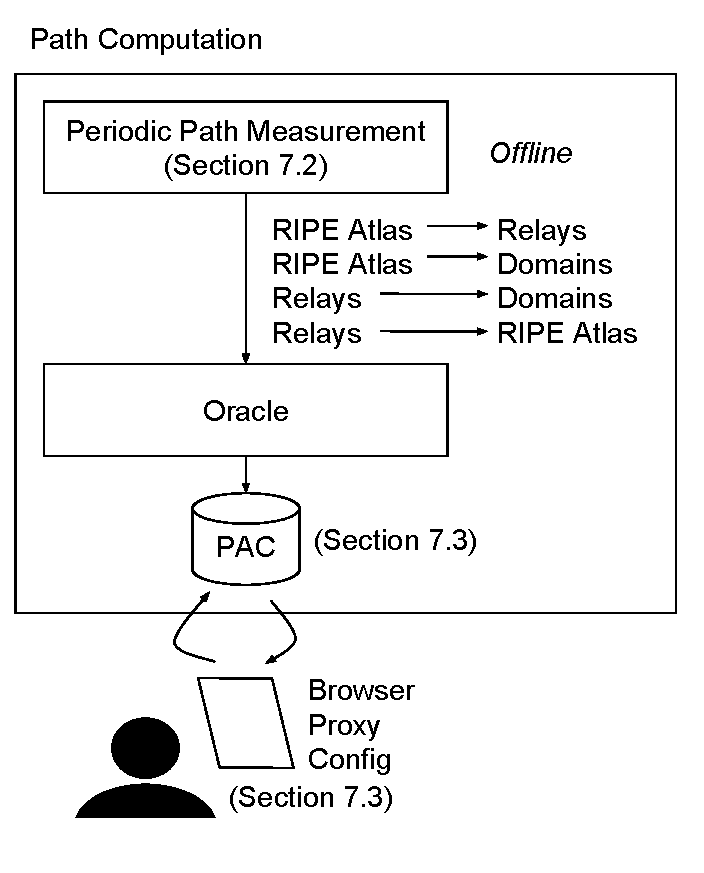
\includegraphics[width=.5\textwidth]{system_overview_updated}
%\caption{\system{} architecture. 1) Paths are computed between clients and relays, 
%relays and domains, relays and clients, and clients and domains.  2) The oracle 
%aggregates all paths.  3)  The oracle generates a PAC file that specifies which 
%domains should be accessed through which relays (based on the measured paths).  
%4) The client configures her browser to use the oracle-generated PAC file.  5) 
%The client's traffic is routed through relays (or direct paths) to access domains, 
%while avoiding a client-specified country.}
%\label{fig:arch}
%\end{figure}

{\bf Design Goals.} Our measurement results motivate 
 the design and implementation of a relay-based avoidance system,
\system{}, with the following design goals.
\label{goals}
\begin{itemize}
\item {\bf Country Avoidance.}  The primary goal of \system{} is to
avoid a given country when accessing web content.  \system{} should
provide clients a way to route around a specified country when
accessing a domain.  This calls for the role of measurement in the
system design and systematizing the measurement methods discussed
earlier in the paper.

\item {\bf Usability.} \system{} should require as little effort as
possible from clients.  Clients should not have to download
or install software, collect any measurements, or understand how the
system works.  This requires a way for clients to automatically and
seamlessly multiplex between relays (proxies) based on different
destinations.  \system{} uses a Proxy Autoconfiguration (PAC) file to support this
function.  PAC files are supported on many types of devices, including mobile 
devices (smartphones, tablets, etc.).  Additionally, this is a mechanism that 
is already being used in systems and tools.  Many Internet users that 
use a VPN have {\it already} used a PAC file; when a user establishes a VPN connection, his 
device's proxy settings are modified to point to a PAC file.  

\item {\bf Scalability.}  This country avoidance system should be able to scale to 
many users.  Therefore, \system{} should be able to handle the addition
 of relays, as well as be cost-effective in terms of resources required. This requires 
clever measurement vantage points, such that each vantage point is representative of 
more than one client.  The PAC file allows \system{} to 
grow with the number of clients and also supports incremental deployment.

\item {\bf Non-goals.}  There are some challenges that \system{} does not
attempt to  solve; in particular, it does not provide anonymity; it routes
around  countries,
but it does not attempt to keep users anonymous in the event that traffic can
be observed.   \system{} also does not address domestic interference or surveillance. For
example, a client in the U.S. cannot use \system{} to avoid network interference 
by the United States. 
\end{itemize}


\subsection{Periodic Path Measurement}

\system{} measures all paths using {\tt 
traceroute}, which is then mapped to the country level using the same methods as 
described in Section~\ref{datasets} and shown in Figure~\ref{fig:analysis_pipeline}.
The paths we measure are the: forward paths from 
the client to each relay; forward paths from each relay to each domain; forward
paths from the client to each domain; and reverse paths from each relay to the 
client. 
%Figure \ref{fig:paths} shows the forward and reverse paths when accessing 
%content using relays; the only path we cannot measure is the reverse path from 
%the domains to the relays because we have no 
%vantage point at or near the domain for running traceroute.
The portion of the reverse path from the domains to the relays is
challenging to measure due to a lack of vantage points in ASes of common
destinations. As discussed in Section \ref{path_sym}, we found that  the
forward and reverse paths are asymmetric at the country level, and therefore
\system{} cannot make any guarantees about which countries are on the path
between  domains and relays even though it has calculated the paths from
relays to domains.   Despite the lack of knowledge about this part of the
reverse path,  we can reason about possible scenarios.  If the client's
traffic is encrypted, then a country on this part of
the reverse path that the client wishes to avoid cannot perform any  traffic correlation
attacks or website
fingerprinting attacks, as the country cannot see who the client is (necessary
for website fingerprinting) and does not have access to more than one part of
the path (necessary for traffic correlation attacks).

\begin{figure}[t!]
    \centering
%    \begin{subfigure}[b]{0.4\textwidth}
        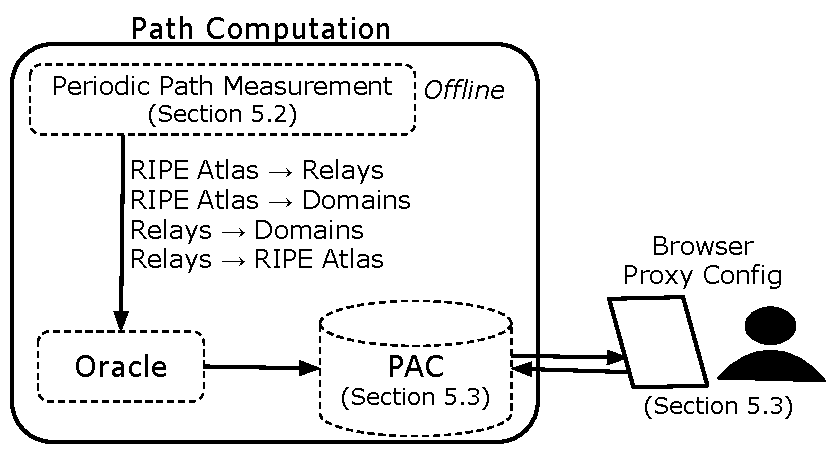
\includegraphics[width=\linewidth]{system_overview_updated-3}
        \caption{\system{} architecture.}
        \label{fig:arch}
%    \end{subfigure}
%    \begin{subfigure}[b]{0.4\textwidth}
%        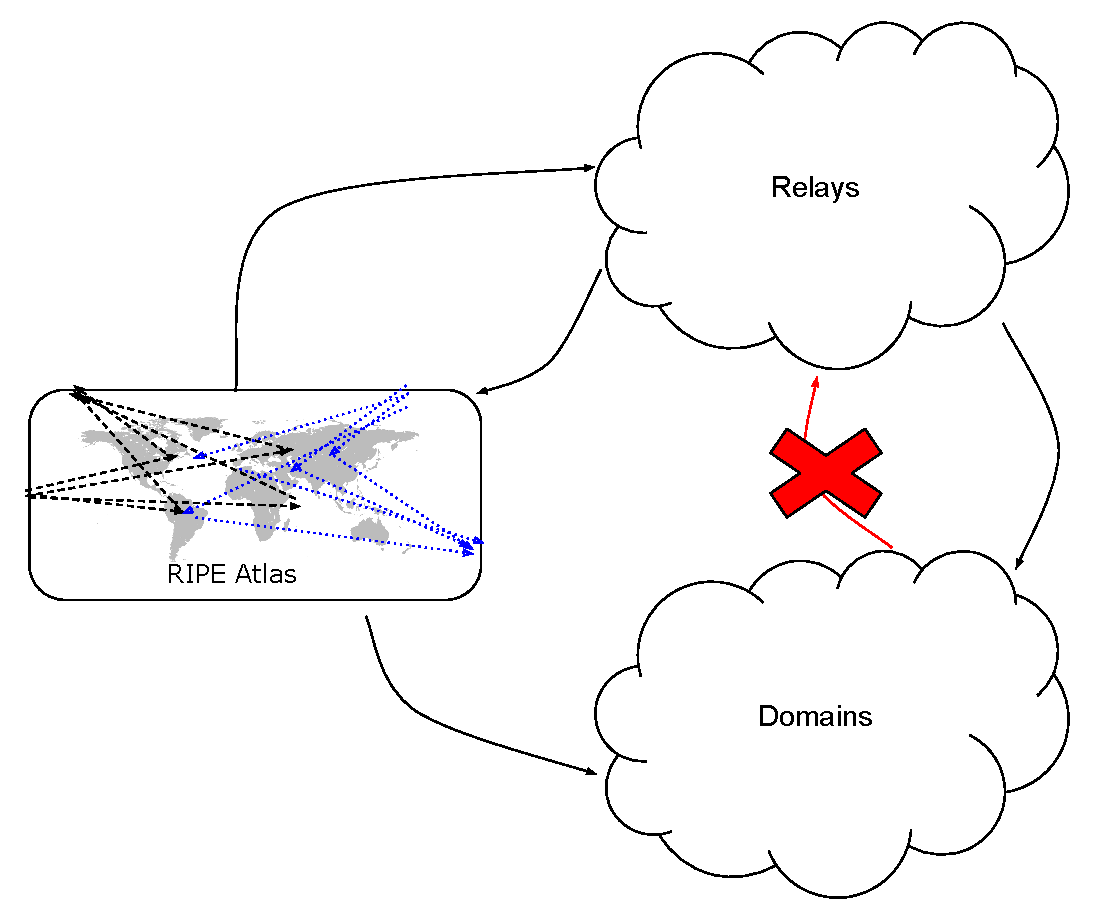
\includegraphics[width=\textwidth,height=7cm]{all_paths}
%        \caption{Paths computed in \system{}.}
%        \label{fig:paths}
%    \end{subfigure}
%    \caption{\system{} architecture, and the path
%      measurements that \system{} periodically computes.}
\end{figure}


\paragraph{Client-to-Relay Paths.} 
To avoid requiring the client to install custom software, \system{}
measures client-to-relay paths from RIPE Atlas probes that serve as 
vantage points for the ASes where \system{} clients might be.  \system{} selects
probes that
are geographically close the client (\eg, in the same 
country). The oracle triggers the probe to run traceroutes
to each relay.  After collecting the responses, the oracle maps 
the IP-level paths to country-level paths and stores the results.

\paragraph{Relay-to-Client Paths.} The \system{} relays perform
traceroutes to the IP addresses of RIPE Atlas probes, which 
represent client ASes.  They then derive country-level paths; the
oracle learns these paths from each relay.  

\paragraph{Relay-to-Server Paths.} Relays perform 
traceroutes to each domain.  As with paths to clients,
relays derive country-level paths and send them to the oracle.

\paragraph{Client to Server Paths.} In case a path from a client to a 
domain does not pass through the country specified to avoid {\it by default}, 
then none of the proxies should be used.  
%If a proxy is used, then it may 
%actually be causing the path to traverse more countries
%(unnecessarily).  
These paths are measured using the RIPE Atlas probes in similar
locations as the clients, and the oracle triggers traceroutes from
each of them to each of the domains.  Corresponding country-level
paths are stored at the oracle.

These paths must be re-computed 
as paths may change.  To our knowledge, there has not been any previous work 
on how often country-level paths change; prior work has explored how often 
AS-level paths change.  We measured the country-level paths from a RIPE Atlas probe to the 
Alexa Top 100 domains once per day for a month to see how stable country-level paths 
are.  Across the measured domains, we found the average time between path changes to 
be about five days.  Therefore, \system{} re-computes the paths every five days to incorporate the 
most recent country-level paths.  

%To measure how often country-level paths change, we 
%computed the paths from relays to domains once every two hours and once every 
%hour.  Fewer than five paths changed every two hours; the 
%results were similar for one-hour increments.  As it takes approximately 30 minutes to 
%compute all paths, \system{} re-computes the paths every one hour to incorporate 
%the most recent country-level paths.

%\begin{figure}[t]
%\centering
%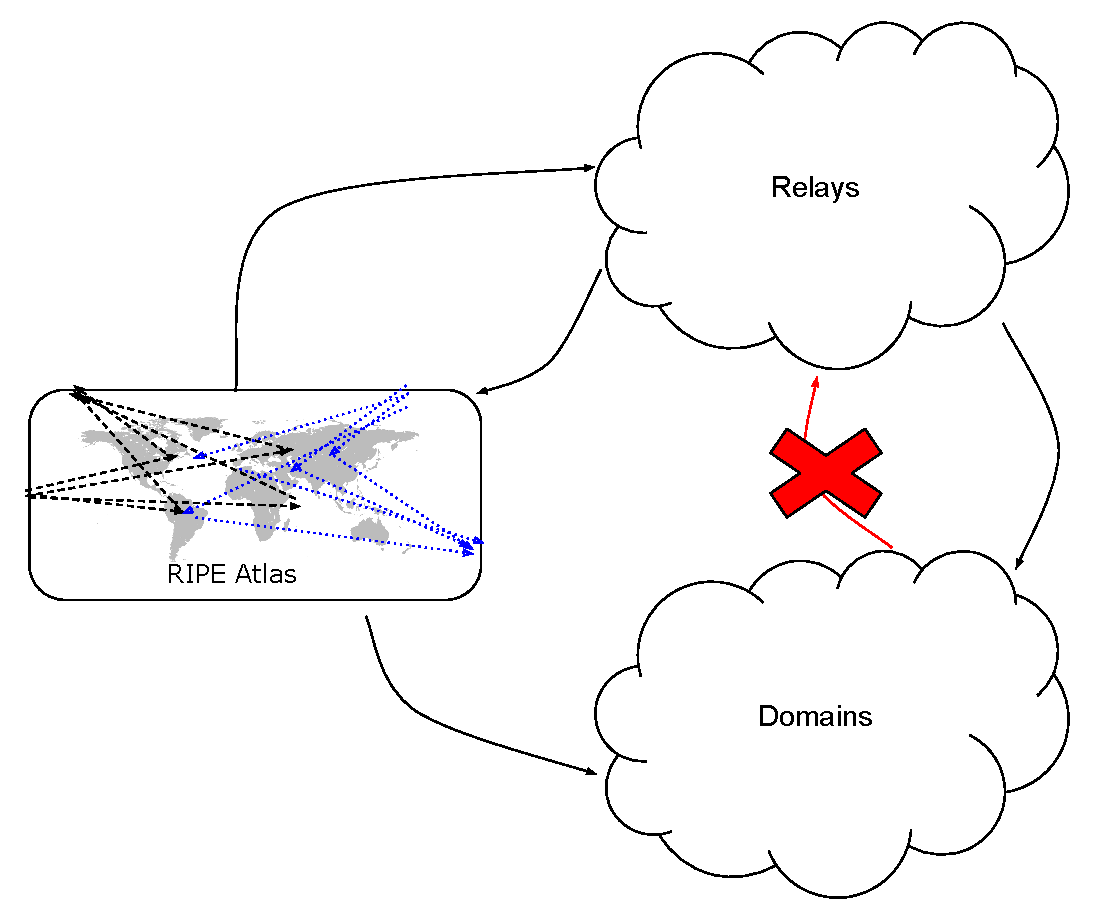
\includegraphics[width=.5\textwidth]{all_paths}
%\caption{The path of a web request through a \system{} relay, to the domain, and back. 
%1) forward path from client to relay; 2) forward path from relay to domain; 3) reverse 
%path from domain to relay; 4) reverse path from relay to client.  \system{} measures 
%all paths except for path 3) due to a lack of vantage points at domain locations.}
%\label{fig:path_components}
%\end{figure}


\subsection{PAC File Generation}
\label{multiplex}
The oracle follows four steps to decide which relay a client should
use to access a specific domain: (1)~If the default path from the
client to the domain does not pass through the specified country, then
do not use any of the relays.  (2)~Otherwise, for all the paths from
the client to the relays, select suitable relays, which are relays where the country 
to avoid is not on the forward or reverse path between the client and 
relay.  (3)~From this set, if there
is a path from a suitable relay to the domain that does not include
the specified country, then use that relay for that domain.  (4)~If
there is no path from the client through any of the relays to the
domain that does not pass through the specified country, then select
the relay that provides the most avoidance (measured by how many other
domains that avoid the specified country).
\begin{figure}[t]
\renewcommand{\lstlistingname}{Configuration}
\lstinputlisting[label={lst:pac}, language=JavaScript, frame=single,
basicstyle=\footnotesize, caption={Example PAC file.}]{example_pac.pac}
\vspace*{-0.25in}
\end{figure}
The oracle applies this decision process to each domain, which results
in a mapping of domains to relays that can be used to avoid the given
country.  To facilitate automatic multiplexing between relays,
\system{} utilizes Proxy Autoconfiguration (PAC) files, which define
how browsers should choose a proxy when fetching a URL.  In the
example PAC file in Configuration~\ref{lst:pac}, proxy 1.2.3.4:3128
should be used when accessing {\tt www.google.com}, but proxy
5.6.7.8:3128 should be used when accessing {\tt www.twitter.com}.  The
oracle uses the mapping of domains to relays to generate a PAC file,
which specifies which domains should be accessed through which proxy.
The PAC file is published online to a URL of the format
$<$client\_country$>$\_$<$country\_to\_avoid$>$\_pac.pac.  The client
uses this URL to specify their proxy configuration.  Paths are
re-computed every five days, so the contents of the PAC file are also
updated every five days.
% The PAC files are published online, which allows a client to simply
% point the proxy configuration settings to the URL that contains the
% PAC file.

\subsection{Scalability and Fault Tolerance}
Adding relays to \system{} is 
straightforward. Additionally, \system{} is resilient to failures of system components.

\paragraph{Adding relays and oracles.} To add a relay, the system
operator must set up a machine as a proxy server, install the relay
software, and update the oracle's list of relays.  From that point
onward, paths will be computed to and from the new relay, and clients
will begin using the new proxy.  Adding an oracle requires installing
the oracle software on a different machine, and specifying the client
locations handled by that oracle (\eg, one oracle handles clients in
North America and Europe, and another handles clients elsewhere).
Both oracles will publish the PAC files to the same server, which
causes no changes for the client.

\paragraph{Failed relays and oracles.} Unresponsive relays are handled
by the PAC file.  The PAC file allows the oracle to specify multiple
proxies in a sequential order, such that if the the first proxy fails,
then the client users the second proxy (and so on).  This feature can
be used to specify all of the relays that have a path to the domain.
%And future work can include relay replicas that can be used in the
%case that a relay crashes.  
Among other mechanisms, we can detect a failed oracle by determining
that its PAC file is older than one hour.  Detecting a failed oracle
could trigger a backup oracle to re-compute the PAC files
periodically.  Because oracles are stateless, failover is
straightforward.  Without backup oracles, clients can still use the
system when the oracle fails.  The clients will simply be using stale
paths, which are likely (but not guaranteed) to be functional, since
country-level paths change infrequently.

\subsection{Security}


\section{Implementation}
Our prototype implementation of \system{} is based on a series of relays, an oracle, and 
a client. All \system{} software can be found at ... \annie{I'll add in wherever we end 
putting it anonymously}

{\bf Relays.}  We established nine relays, one in each of the following countries: Brazil, 
Germany, Singapore, Japan, Australia, France, United States, United Kingdom, and Canada.  
They are running as Ubuntu Virtual Private Servers (VPSs) with 
Squid as the proxy server.  It is also running the \system{} Relay software.

\begin{figure}[b!]
\centering
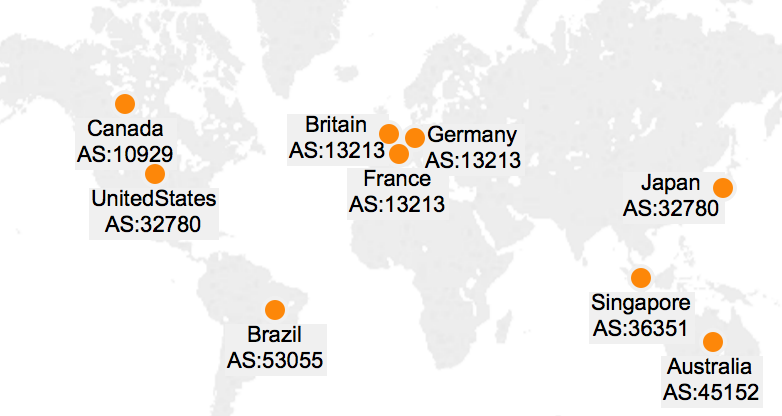
\includegraphics[width=.5\textwidth]{relay_map}
\caption{}
\label{fig:relay_locations}
\end{figure}

{\bf Oracle.}  The oracle is a Fujitsu RX200 S8 server with dual, 
eight-core 2.8GHz Intel Xeon E5 2680 v2 processors with 256GB RAM running the 
Springdale distribution of Linux. It is running the \system{} Oracle software.

{\bf Client.} For the purposes of the system evaluation, we set up a client 
machine in the Netherlands, which simply accesses web content and uses the PAC 
file.

\lstinputlisting[label={lst:pac}, language=JavaScript, frame=single, basicstyle=\footnotesize, caption={An example PAC file.}]{example_pac.pac}

\section{Evaluation}
Using the \system{} implementation, we evaluate the system on it's ability to avoid a given country, performance, and scalability in terms of storage and costs.

\subsection{Country Avoidance}
As the primary goal of the system is to provide country avoidance for a given 
country, we measured how much avoidance the system achieves.  We did so by first 
calculating the number of {\it default} paths that avoid a given country.  Then 
we added a single relay, and calculated how many domains the client could 
access without traversing through the given country.  This was repeated for 
the remaining two relays.  The evaluation was conducted under the condition that 
the client wished to avoid different countries when accessing the Netherlands top 
100 domains, and the results are shown in Figure \ref{fig:avoidance_eval}.  Each 
line represents the fraction of domains accessible while avoiding the country that 
the line represents.  For example, 46\% of domains are accessible without traversing 
the United States when \system{} is not being used (0 relays), and if \system{} is 
used, then 63\% of domains are accessible with traversing the United States.

\begin{figure}[b!]
\centering
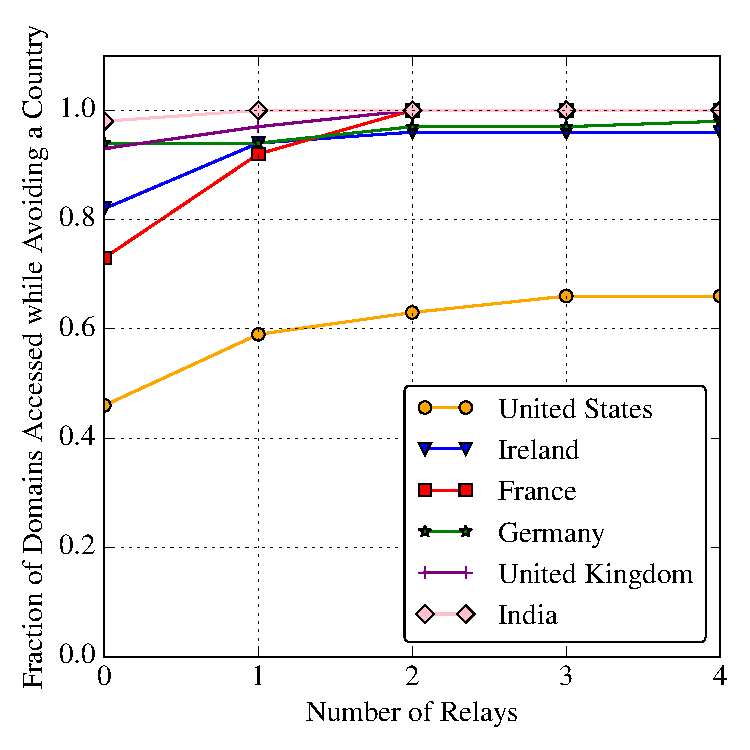
\includegraphics[width=.5\textwidth]{avoidance_n_relays}
\caption{How much avoidance different numbers and locations of relays achieve.}
\label{fig:avoidance_eval}
\end{figure}

It is evident that \system{} helps a client avoid a foreign country, as the 
fraction of domains accessible without traversing 
the specified country without \system{} is lower than with \system{}.  Additionally, 
it is clear that adding the first relay provides the greatest increase in 
provided avoidance, while subsequent relays provide a significantly 
smaller amount (or no) additional avoidance.

Figure \ref{fig:avoidance_eval} also clearly shows how much more difficult (or 
impossible) it is to avoid the United States than it is to avoid any other 
country.  Only 63\% of domains can be accessed while avoiding the United States, 
whereas almost all domains can be accessed while avoiding any other given 
country.  This confirms the results presented in Section \ref{avoid_results}, and 
emphasizes how crucial the systematization of the measurements is for enabling 
\system{}.

\subsection{Performance}
A system is not usable if the performance is significantly worse than what a user
is accustomed to.  To measure the performance of \system{}, we measure both 
the throughput and latency.

To measure throughput, we ran {\tt wget} for each 
of the top 100 domains from the client machine in the Netherlands, while 
using the PAC file.  Based on the {\tt wget} output, we calculate the number 
of seconds to access content using our system. Figure \ref{fig:latency} shows 
the CDF of the ratio of direct throughput to \system{} throughput. 

\begin{figure}[t]
\centering
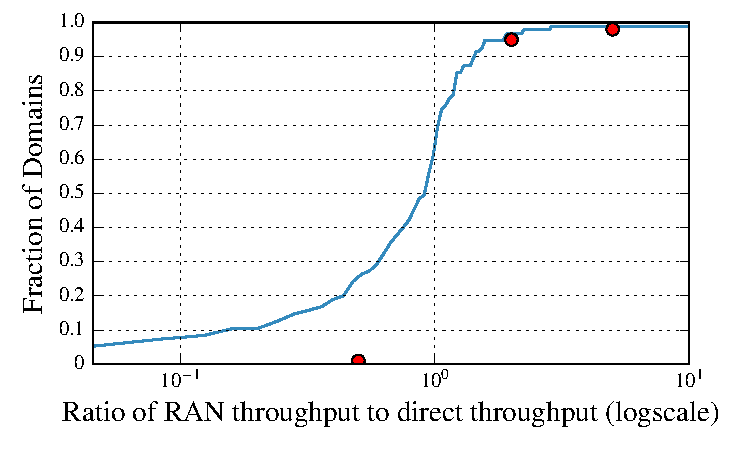
\includegraphics[width=.5\textwidth]{throughput}
\caption{Latency difference when accessing a webpage via \system{} vs. default paths. 
The difference is calculated by \system{} latency minus default latency, and represents 
the additional latency cost of our system.}
\label{fig:latency}
\end{figure}

We can see that the throughput of \system{} is not significantly worse than that 
of default paths.  In fact, in some cases the performance of \system{} is {\it 
better} than that of default paths.  This could be a result of the relays 
keeping local traffic local, or due to a closer content replica being selected. 
These results show that \system{}'s performance is comparable to the performance 
of accessing domains without \system{}.

To measure the latency of \system{}, we ran a {\tt curl} command to each of the 
top 100 domains from the client machine in the Netherlands, while using the PAC file. 
This provided the time to first byte (TTFB); we found the TTFB for both \system{} and 
direct paths, and the results are shown in Figure \ref{fig:latency}.  

\begin{figure}[t]
\centering
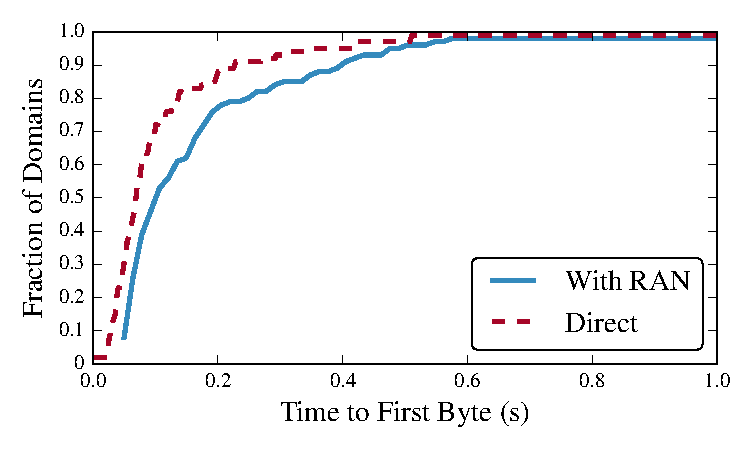
\includegraphics[width=.5\textwidth]{latency}
\caption{Latency difference when accessing a webpage via \system{} vs. default paths. 
The difference is calculated by \system{} latency minus default latency, and represents 
the additional latency cost of our system.}
\label{fig:latency}
\end{figure}

The median TTFB for direct paths is .0685, and for \system{} paths, it is .10075.  Additionally, 
the 90th percentile for direct and \system{} paths is .2253 and .40352, respectively.  This 
shows that the system's latency is greater by a factor of 2 (or 20-40ms).  \annie{Say if this is 
significant or not, especially as it relates to page load times.}

\subsection{Storage}
As the number of clients increase, and subsequently the number of paths being 
computed increases, the amount of storage must remain reasonable.  The storage 
used by paths can be calculated:

\[Storage(D,R,C) = (D x R) + 2(C x R) + (C x D) \]

D is the number of domains; R is the number of relays; C is representative of the number of 
clients.  While C {\it represents} clients, it is not the number of clients using the 
system --- it is the number of vantage points the system uses to measure paths 
from client locations.  For the prototype with a single client, the storage space for all 
paths computed is 480KB.  As there is a single PAC file for all clients in 
a country, C will grow much slower than if there was a different PAC file for 
each individual client.  There are 196 countries in the world today, and if 
paths and a PAC file were generated for each country, with 100 domains, and 
three relays, the storage would only be 94MB.  This provides plenty of storage 
for increasing the number of domains included in the PAC file or increasing 
the number of relays in the system.

\subsection{Costs}
In addition to storage, the cost of the measurements used in the system must 
be taken into account.  RIPE Atlas credits are a limited resource, and therefore 
we must earn more credits than we are spending on measurements.  The cost 
in credits follows the equation:

\[Credit\_Cost(D,R,C) = COST_{traceroute}((C x R) + (C x D))\]

Currently, the $COST_{traceroute}$ is 60, resulting in a prototype cost of 6,180 
credits, but because these paths are updated each hour, then 
the daily credit cost is 148,320 credits.  In return for hosting a RIPE Atlas 
probe, we earn 216,000 credits per day, which will support our existing 
prototype.  In order to provide for more clients, more domains, or more 
resources, we can tune the system to re-compute paths less frequently (only when necessary).

\section{Conclusion}
\label{conclusion}

We have characterized routing
detours that take Internet paths through foreign countries, showing 
that underserved regions often depend on the United States and Europe to 
access popular content; this can cause performance degradation, increased costs, 
and gives more power to these dominant countries to perform surveillance and censorship.   %we have
%investigated how clients, ISPs, and governments can use overlay network relays to prevent routing detours through
%a given country.  This method gives clients the power to
%avoid certain countries, as well as help keep local traffic local.
%Although some countries are completely avoidable, we find that some of
%the more prominent surveillance states are the least avoidable.
As a first step towards a remedy, we have
designed, implemented, and deployed \system{}, which employs overlay network
relays to  route traffic around a given country; our data and code is publicly available~\cite{ransom_data,ran_system}.  %Our evaluation
%shows  that \system{} can in many cases avoid certain countries while
%performing nearly as well, if not better, than taking default routes.

%Our work presents several opportunities for follow-up studies and
%future work. First, Internet paths continually
%evolve; we will repeat this analysis over time and publish the results
%and data on a public website, to help deepen our collective
%understanding about how the evolution of Internet connectivity affects
%transnational routes. Second, our analysis should be extended to study
%the extent to which citizens in one country can avoid groups of
%countries or even entire regions. Finally, although our results provide strong 
%evidence for the existence of various transnational data flows, factors
%such as uncertain IP geolocation make it difficult to provide clients
%guarantees about country-level avoidance; developing techniques and
%systems that offer clients stronger guarantees
%is a ripe opportunity for future work.


\bibliographystyle{abbrv}
\bibliography{sigproc}

\end{document}
